
\section[Clipping Without Materializing Per-Example Gradients]{\large Clipping Without Materializing Per-Example Gradients}
DP-SGD has high memory overhead due to clipping \textit{per-example} gradients.
Na\"ively implemented, this step instantiates a giant gradient vector for each example during optimization and can be prohibitively expensive.
For example, \cite{hoory2021learning} pretrained BERT with DP optimization and reported memory issues when using the large batches necessary to achieve high performance.
A time-costly solution to the memory problem is micro-batching: Split large batches into multiple smaller ones and aggregate the results after processing each small batch individually~\citep{tramer2020differentially}.
This solution, however, is unlikely to be sufficient as neural language models become larger and fitting even a few copies of the gradient in memory can be difficult.
\cite{lee2020scaling} observed that per-example gradients need not be instantiated at all, if the goal is to sum the clipped gradients. 
They presented a clipping procedure that only instantiates the per-example gradient for parameters of a \textit{single} layer in the model one at a time, as opposed to the entire model at once, at the cost of an extra backpropagation pass per processed batch. 


Unfortunately, we find this trick to be still insufficient for sequence models such as Transformers~\citep{vaswani2017attention}, as the memory requirement for per-example gradients of embedding layers and language modeling heads can be costly. We extend the \cite{lee2020scaling} approach such that training Transformers with DP optimization can have almost the same memory consumption as non-private training. 
Unlike their approach, our extension avoids instantiating the per-example gradient even for individual linear layers.
We call this approach \textit{ghost clipping}, as the per-example gradient is the ghost that never explicitly appears.
We anticipate this extension to be useful for both privately fine-tuning and pretraining large Transformers.

\subsection{The Memory Trick By~\cite{lee2020scaling}}
Per-example gradient clipping is easy if we know per-example gradient norms. In this case, we first compute the scaling factor $c_i = \min(1, \nicefrac{C}{ \normtwo{ \nabla \mathcal{L}_i} })$, where $C$ is the clipping threshold and $\mathcal{L}_i$ is the loss associated with the $i$th example. Then, we perform the usual backward pass with the reweighted scalar loss $ \sum_{i} c_i \mathcal{L}_i $. This procedure gives us the sum of clipped gradients.
Under this setup, the difficulty is computing the per-example gradient norm $\normtwo{\nabla \mathcal{L}_i}$. 
We emphasize two technicalities that enable computing this quantity without instantiating the full per-example gradient $\nabla \mathcal{L}_i$. 

First, for a typical neural net layer $l$ with parameters $W^{(l)}$ (without parameter sharing), the per-example gradient w.r.t. parameters can be easily computed using the input to the layer $a^{(l)}$ and the gradient of the loss w.r.t. the output $g^{(l)}$, both of which are available during backpropagation. 
Second, for a large vector formed by concatenating several small vectors $u = [u_1, \dots, u_k]$, its Euclidean norm is simply the norm of the vector of norms, i.e. 
$
\normtwo{ u } =
    \normtwo{ ( \normtwo{u_1}, \dots, \normtwo{u_k} ) }. 
$
The second observation means that computing the per-example gradient norm $\normtwo{\nabla  \mathcal{L}_i}$ can be done by computing the per-example gradient norms for individual layers of the neural net $\normtwo{\nabla_{W^{(1)}}  \mathcal{L}_i}, \dots, \normtwo{\nabla_{W^{(L)}}  \mathcal{L}_i}$ one at a time ($L$ is layer count). 
Moreover, the first observation implies that the norms for each layer can be computed using quantities freely available to a typical backward pass.
Overall, the per-example gradient norm of any network without parameter sharing can be computed in a layer-by-layer fashion with only one per-example gradient tensor for a single layer being instantiated at any time. 




\subsection{Ghost Clipping for Transformers With Sequential Data}\label{sec:our_ghost}
The trick by~\cite{lee2020scaling} still requires instantiating the per-example gradient of individual layers (although not simultaneously). 
This can be problematic in terms of memory for Transformers with large embedding layers.\footnote{
	For GPT-2, per-example gradients w.r.t. the embedding for ten examples alone occupy \mytextapprox{1.5}GB of memory.
} 
Here, we present a specialized procedure for computing the per-example gradient norm for linear and embedding layers when they are applied to sequential data.\footnote{An embedding layer is essentially a linear layer: The embedding lookup operation applied to indices is equivalent to a matrix multiplication of the embedding matrix with one-hot encoded indices.}
This procedure reduces memory footprint and can be viewed as a generalization of the \cite{goodfellow2015efficient} trick that additionally handles sequential inputs. 

Let $a \in \R^{B\times T \times d}$ be the input to a linear layer with weight matrix $W \in \R^{p \times d}$, and $s \in \R^{B \times T \times p}$ be the output with $s_{i, j} = W a_{i, j}$. Let $g \in \R^{B \times T \times p}$ be the gradient of the loss w.r.t. the output $s$. 
Here, $T$ is the number of time steps in the input, and we omitted biases for simplicity. 
Simple calculation shows that the per-example gradient is the product of two matrices:
\eq{
\label{eq:seq_per_example_grad}
\nabla_{W} \mathcal{L}_i = g_i^\top a_i \in \R^{p \times d}. 
}
Since the per-example gradient norms are the end goal, the per-example gradients $\{\nabla_W \mathcal{L}_i\}_{i=1}^B$ themselves need not be instantiated explicitly. 
More precisely, we observe that the squared per-example gradient norm for this layer $\normf{\nabla_{W} \mathcal{L}_i}^2$ obeys the following key identity:
\eq{
\label{eq:better_per_example_grad}
\normf{ \nabla_{W} \mathcal{L}_i }^2 =
    \mathrm{vec}(a_{i} a_{i}^\top)^\top \mathrm{vec}( g_i g_i^\top ).
}
See Appendix~\ref{app:frobenius} for a derivation. 
Implemented with common primitives in machine learning libraries, \eqref{eq:better_per_example_grad} has a memory complexity of order $\mathcal{O}(BT^2)$ when $a_{i} a_{i}^\top\in\R^{T\times T}$ and $g_{i} g_{i}^\top\in\R^{T\times T}$ are instantiated,\footnote{The derived complexity is based on the assumption that the space complexity for multiplying two matrices $A\in \R^{m\times n}$ and $B\in \R^{n\times p}$ is roughly $\mathcal{O}(mp)$, which is the case for most workloads running on a framework like PyTorch. 
In addition, more sophisticated solutions may even avoid instantiating $a_{i} a_{i}^\top$ and $g_{i} g_{i}^\top$ entirely by trading in more run-time. Custom CUDA kernels are likely needed to make these solutions fast in practice.
} as opposed to $\mathcal{O}(Bpd)$ in the na\"ive approach which goes through instantiating \eqref{eq:seq_per_example_grad}.\footnote{We omitted the cost of storing $a_i$ and $g_i$, since our goal is to compare the additional cost induced by computing gradient norms.}

The memory efficiency of this procedure is exemplified with off-the-shelf pretrained language models, most of which have large embedding layers. 
For instance, for GPT-2, $d\approx50,000$ and $p=768$ for the embedding layer, and the context window $T\le 1024$.\footnote{In practice, for fine-tuning tasks, the maximum sequence length is usually a few hundred. } 
Our method in theory reduces the memory cost associated with this large embedding layer by at least a factor of $22$ compared to when the per-example gradient is na\"ively instantiated.
Overall, we also observe significant savings, since embedding layers can be a major source of memory spending for training large language models.\footnote{While there are alternative approaches for reducing the memory footprint of embedding layers during training,  
these methods tend to introduce extra hyperparameters that potentially require further tuning and privacy spending.
}

To stress-test ghost clipping, we compare it with $4$ baselines: The \texttt{PyTorch} package \texttt{Opacus} that implements DP optimization by instantiating per-example gradients, the approach by \cite{lee2020scaling}, non-private training in \texttt{PyTorch}, and na\"ive DP optimization implemented in \texttt{JAX} with \texttt{jit} and \texttt{vmap} enabled. 
We include the \texttt{JAX} baseline since a recent study showed that DP optimization can be made cheap through compiler optimization~\citep{subramani2020enabling}.
Figure~\ref{fig:ghost_clipping} (a) shows that for typical inputs, our technique is the most memory friendly and allows fitting batches almost as large as those in non-private training. 
Since ghost clipping allows us to fit larger batches but with a run-time penalty, a natural question is whether it improves throughput with the use of larger batches. 
Figure~\ref{fig:ghost_clipping} (b) shows that while ghost clipping only provides minor gains compared to \texttt{Opacus} for smaller models, it allows processing \mytextapprox{10\%} more examples compared to the approach by~\cite{lee2020scaling} for fitting GPT-2-large, a model that neither \texttt{Opacus} or \texttt{JAX} could handle. 
% See Appendix~\ref{app:memory} for the setup of these experiments.
\begin{figure}[htb]
\begin{center}
\begin{minipage}[t]{0.48\linewidth}
\centering
{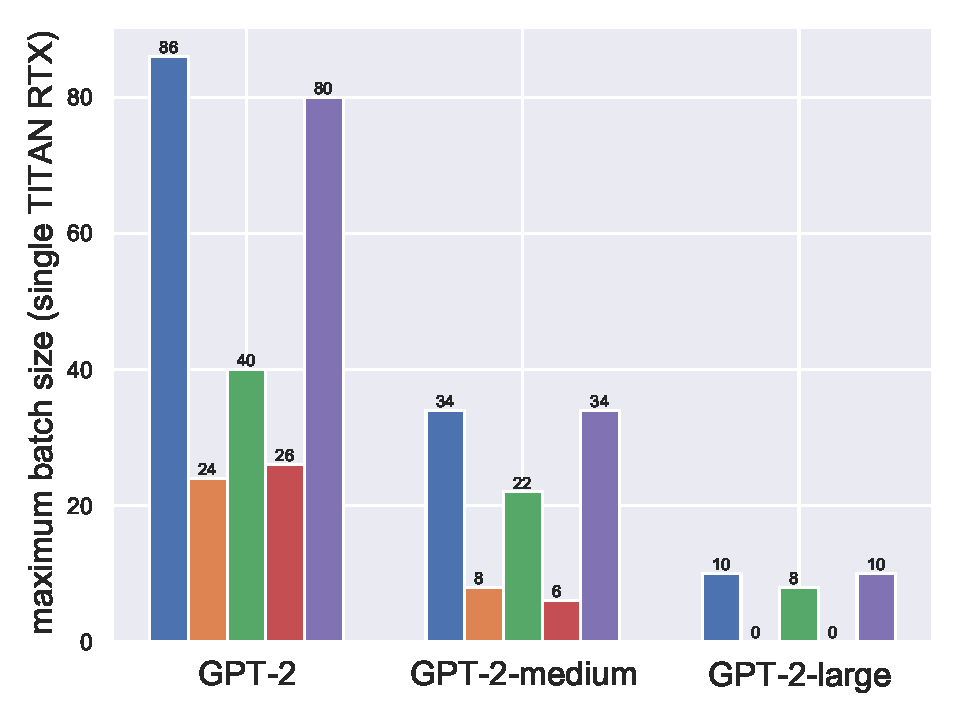
\includegraphics[width=0.98\textwidth]{figs/mem.pdf}}
(a) Memory
\end{minipage}
\begin{minipage}[t]{0.48\linewidth}
\centering
{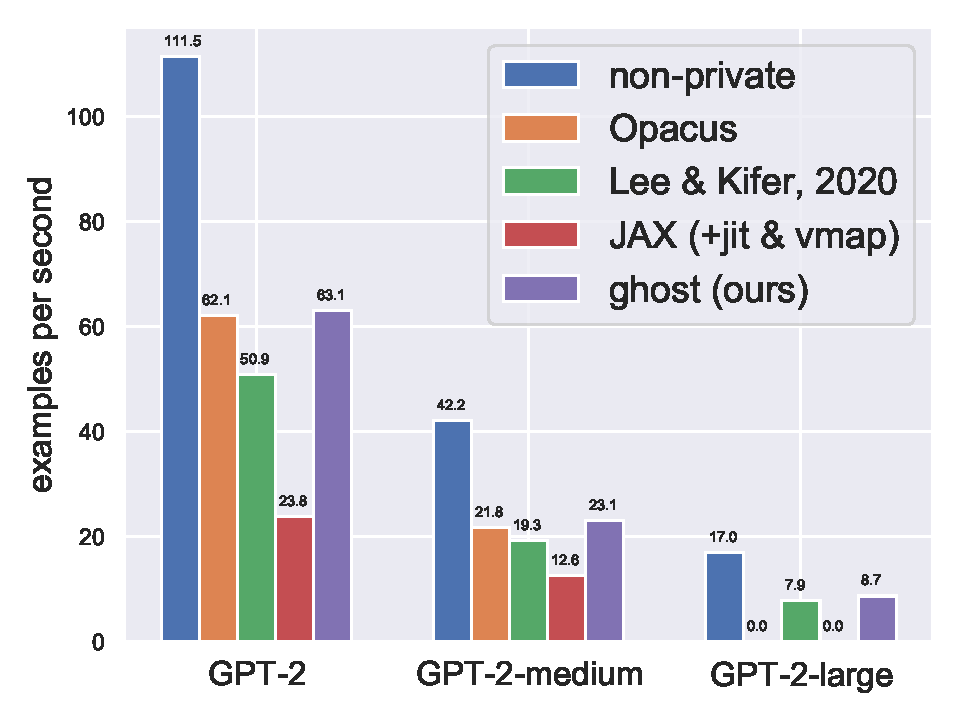
\includegraphics[width=0.98\textwidth]{figs/throughput.pdf}} 
(b) Throughput
\end{minipage}
\end{center}
\caption{
\textbf{Left:} 
Ghost clipping is 3 times more memory efficient than \texttt{Opacus} and is almost as efficient as non-private training for typical sequences across model sizes.
For GPT-2-large, we were unable to fit single-example micro batches together with gradient accumulation with \texttt{Opacus} or \texttt{JAX} on a TITAN RTX GPU ($24$ GBs of VRAM).
\textbf{Right:} DP optimization with ghost clipping processes \mytextapprox{10\%} more examples than the approach by~\cite{lee2020scaling} under unit time for GPT-2-large.
}
\label{fig:ghost_clipping}
\end{figure}
